\documentclass[fleqn]{jbook}
\usepackage{physpub}

\begin{document}

\begin{question}{専攻 問題7}{}


\begin{subquestions}
\SubQuestion
  細胞内での拡散過程による物質輸送は、移動距離が短いときは、他の生物的
  な反応速度などと比べて十分速いが、移動距離が長くなるにつれ、急激に遅
  くなる。このことを半定量的に示すために、次のような場合を考察しよう。

  真核生物の細胞の典型的な大きさは $20\Unit{\mu m}$ であり、原核生物
  (バクテリアなど)の典型的な大きさは $1\Unit{\mu m}$ である。典型的な
  タンパク質分子(拡散定数:$10^{-7}\Unit{cm^2/s}$) がそれぞれの細胞の
  なかで、細胞の大きさである $1\Unit{\mu m}$ だけ、一次元的な拡散に
  よって移動するのに必要な時間を概算せよ。


\SubQuestion
  神経細胞は細胞体・樹状突起・軸索からなるが、軸索の長さは$1\Unit{m}$
  である場合もある。その場合は、細胞体で合成されたタンパク質が一次元的
  な拡散で軸索の先端に達する時間は、典型的なタンパク質では約1600年かか
  ることが上記と同様な概算の結果わかるので、物質輸送を拡散過程に頼る
  ことは出来ないことは明白である。

  このような状況に対処するために真核細胞では特別な機能を持つタンパク質
  のシステムがいくつか出現した。それらを簡単に列記し、そのうちの一つに
  関しては、そのシステムを構成するタンパク質とその特性についても触れ
  つつ、詳しく述べよ。

\end{subquestions}
\end{question}
\begin{answer}{専攻 問題7}{}


\begin{subanswers}
\SubAnswer
  拡散方程式は$t=0$で$x=0$にあった分子の$t$秒後の分布$f(x,t)$に対し、
%
  \[ \Partial{f}{t} = D\Partial{^2 f}{x^2} \qquad (D:拡散定数) \]
%上式改訂
%
  となる。この解は、初期条件$f(x,0)=\delta(x)$の下で、
%
  \[ f(x,t) = \frac{1}{\sqrt{4\pi Dt}} e^{-\frac{x^2}{4Dt}} \]
%
  で与えられる。これから、$t$秒後の分子の平均移動距離
  $\sqrt{\Mean{x^2}}$を求めると、
%
  \[ \Mean{x^2} = \Iint{\d{x}} x^{2}f(x,t) = 2Dt \hspace{15mm}%
     \Yueni \sqrt{\Mean{x^2}} = \sqrt{2Dt} \]
%
  これに、$x=1[\Unit{\mu m}]$、$D=10^{-7}[\Unit{cm^2/s}]$ を代入すると、
%
  \[ t = 5 \Keta{-2} [\Unit{s}] = 50[\Unit{ms}] \]
%
  一方、$x=20[\Unit{\mu m}]$ の場合、$t=20[\Unit{s}]$である。


\SubAnswer

    軸索輸送をするタンパク質には kinesin、dynein、tau protein がある。 
  kinesinとcytoplasmic dyneinによる軸索(axon)輸送について説明する。

%  \begin{minipage}{105mm}

  神経細胞の軸索には微小管(microtubule)が通っていて、これに沿って軸索
  輸送が行なわれる。微小管は極性を持っていて、軸索内では細胞体側が
  $-$endになっていて、シナプス側が$+$endになっている。

 \bigskip
 
 \begin{minipage}{105mm}
  \begin{center}
    \fbox{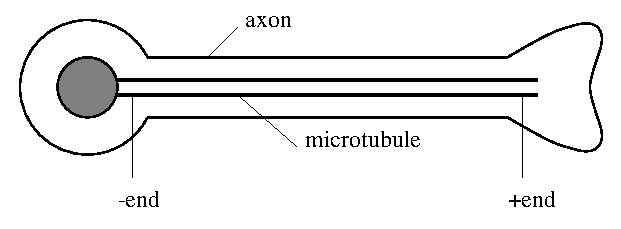
\includegraphics[clip]{1995phy7-1.eps}}
  \end{center}

  kinesinは右図のように微小管にbindする部分と運ぶ細胞内の
  物質にbindする部分をもち、ATPを分解することにより、
  $+$end方向に移動する。一方、dyneinはkinesinとは逆方向の
  $-$endに向かって移動する。よって、kinesinとdyneinによって
  相補的に軸索輸送は行なわれる。

  \end{minipage}
  \begin{minipage}{55mm}
  \begin{center}
    \fbox{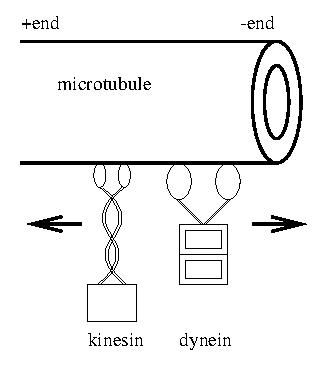
\includegraphics[clip]{1995phy7-2.eps}}
  \end{center}
  \end{minipage}

\end{subanswers}
\end{answer}


\end{document}
